\documentclass[11pt, oneside]{article} 
\usepackage{geometry}
\geometry{letterpaper} 
\usepackage{graphicx}
	
\usepackage{amssymb}
\usepackage{amsmath}
\usepackage{parskip}
\usepackage{color}
\usepackage{hyperref}

\graphicspath{{/Users/telliott/Github/Tex/png/}}
% \begin{center} 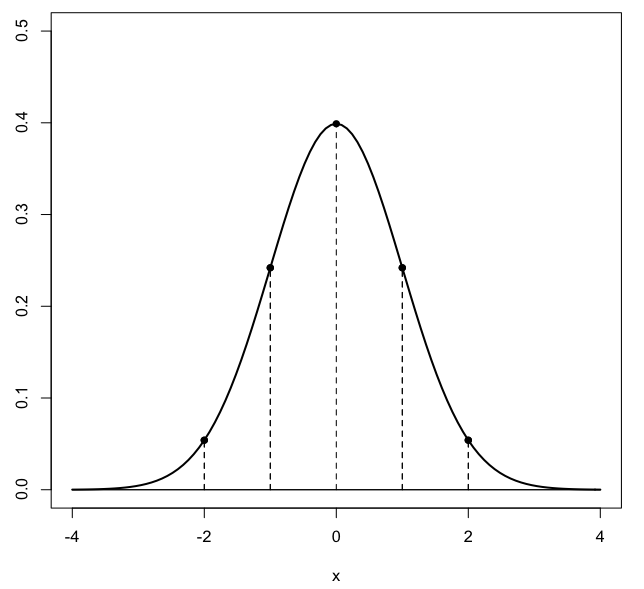
\includegraphics [scale=0.4] {gauss3.png} \end{center}

\title{Theorems}
\date{}

\begin{document}
\maketitle
\Large

We say that a function $f$ approaches the \textbf{limit} $L$ near $a$ if, for every $\epsilon > 0$ there exists $\delta > 0$ such that for all
\[ 0 < |x - a| < \delta \]
implies
\[ |f(x) - L| < \epsilon \]

And we say that a function is \textbf{continuous} at $a$ if 
\[ \lim_{x \rightarrow a} f(x) = f(a) \]

\subsection*{preliminary theorem}

Suppose $f$ is continuous at $a$ and that $f(a) > 0$.  Then $f(x) > 0$ for all $x$ in some interval containing $a$.  More precisely, there is a number $\delta > 0$ such that $f(x) > 0$ for all $x$ satisfying $|x-a| < \delta$, that is, all $x$ in $[a - \delta, a + \delta]$.

\subsection*{proof}

Since $f$ is continuous, for every $\epsilon > 0$ there is a $\delta > 0$ such that for all $x$ satisfying $|x - a| < \delta$, then $|f(x) - f(a)| < \epsilon$.
\[ -\epsilon < f(x) - f(a) < \epsilon \]

This must be true for $\epsilon = f(a)$ (since $f(a) > 0$).  Hence
\[ - f(a) < f(x) - f(a) < f(a) \]
so
\[ f(x) > 0 \]

\section{Bolzano's Theorem}

\subsection*{theorem}

If $f$ is continuous on $[a,b]$ and $f(a) < 0 < f(b)$ then there is some $x$ in $[a,b]$ such that $f(x) = 0$.

\begin{center} 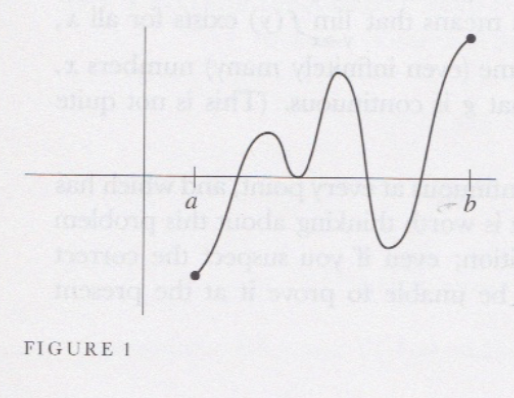
\includegraphics [scale=0.35] {spivak1.png} \end{center}

\subsection*{Spivak}

Recall the completeness axiom in this formulation:  if $A$ is a set of real numbers, $A \ne \varnothing$, and A is bounded above, then A has a \emph{least upper bound}.

Define $A = \{ \ x: a \le x \le b$ and $f$ is negative on $[a,x] \ \}$.  

\begin{center} 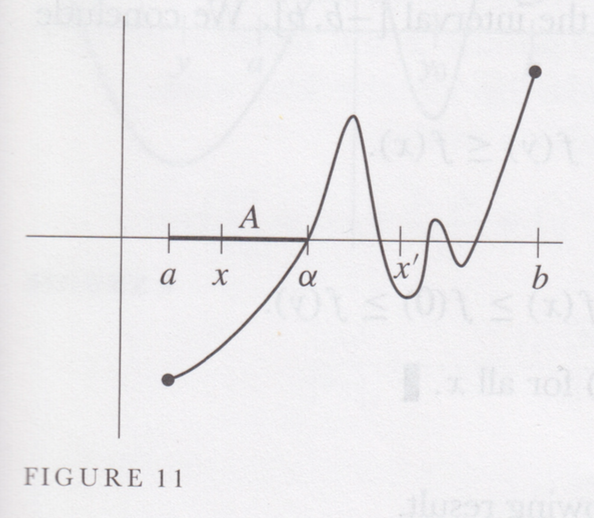
\includegraphics [scale=0.35] {SpivakIVT1.png} \end{center}

(This definition of $A$ will exclude points like $x'$ where $f(x') < 0$, but not every point in $[a,x']$ is $< 0$.  In effect, we are focusing on the first time $f(x)$ crosses zero.  We prove there is at least one such $x$).

Clearly, $a \in A$ since $f(a) < 0$, so $A \ne \varnothing$.  

Since $f$ is continuous, points $x$ close to $a$ also have the property that $f(x) < 0$.

Similarly $b \notin A$ and points near $b$ have the property that $f(x) > 0$ and so these points are also not in $A$.  Hence $b$ is certainly an upper bound for $A$.  

Therefore, by the completeness axiom, $A$ has a least upper bound.  Let us call it $\alpha$.  

We claim that $f(\alpha) = 0$.  The proof is by contradiction.

\subsection*{proof}

$\circ$  Suppose $f(\alpha) < 0$

\begin{center} 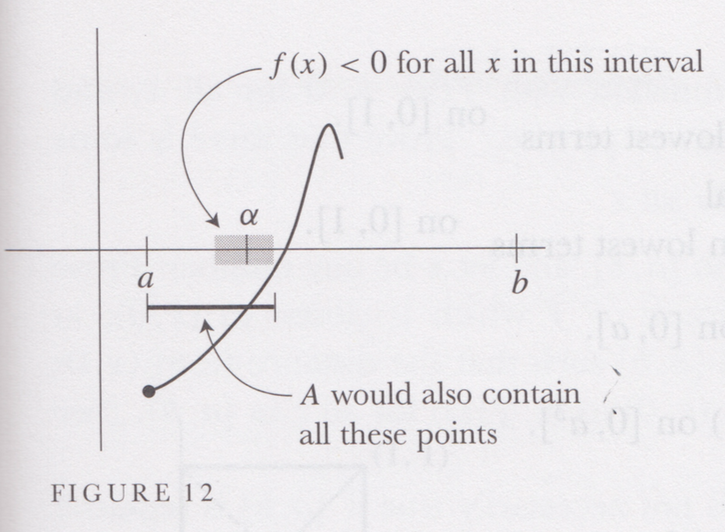
\includegraphics [scale=0.35] {SpivakIVT2.png} \end{center}

If $f(\alpha) < 0$ then nearby points also have this property.  In particular we can find $\delta$ such that if $x$ is in $[\alpha, \alpha + \delta]$, $f(x) < 0$. But this contradicts the fact that $\alpha$ is an upper bound for $A$, since there would be points $x > \alpha$ that are in $A$.

$\circ$  Suppose $f(\alpha) > 0$

If $f(\alpha) > 0$ then points in the neighborhood of $x$ also have this property.  

\begin{center} 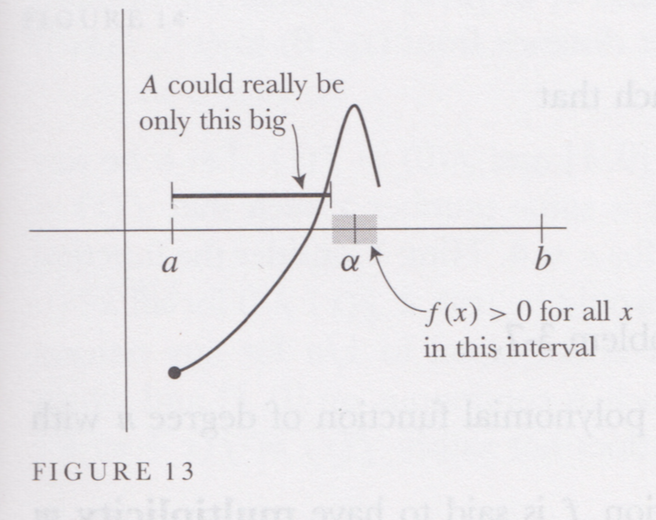
\includegraphics [scale=0.35] {SpivakIVT3.png} \end{center}

In particular we can find $\delta$ such that if $x$ is in $[\alpha - \delta, \alpha]$, $f(x) > 0$. But this contradicts the fact that $\alpha$ is the least upper bound for $A$, since there would be points $x < \alpha$ that are not in $A$ and so also upper bounds.

$\square$

I found another version of this proof with the same logic but with more $\delta$ and $\epsilon$ stuff.

\subsection*{proof}

We look for the largest $x$ on this interval such that $f(x) \le 0$.

$\circ$  Let $\mathbf{S}$ be the set of all $x \in [a,b]$ such that $f(x) \le 0$.  

$\circ$  $\mathbf{S}$ is non-empty ($\mathbf{S} \ne \varnothing$) since $a \in \mathbf{S}$.  

$\circ$  Since $f(b) > 0$, $b \notin \mathbf{S}$, and since every $x$ in the relevant interval is $\le b$, $b$ is larger than all members of $\mathbf{S}$, and so $b$ is an upper bound of $\mathbf{S}$.

The completeness axiom says that every non-empty subset of $\mathbb{R}$ that is bounded above has a supremum in $\mathbb{R}$.

$\circ$  Therefore, by the property of \textbf{completeness}, there exists a least upper bound or supremum of $\mathbf{S}$. 

$\circ$  Define $c$ to be that supremum, the largest $x$ in this interval with the property that $f(x) \le 0$.

$\circ$  Since $f(x)$ is continuous, $\lim_{x \rightarrow c} f(x) = f(c)$.

\noindent\rule{2cm}{0.4pt}

Exactly one of three things is true:  $f(c) > 0, f(c) < 0$ or $f(c) = 0$.  

We claim that $f(c) = 0$.  The proof is by contradiction.  

Suppose $f(c) > 0$.

$\circ$  We define $\epsilon_1 = f(c)/2$.  Then $\epsilon_1$ is positive and $2 \epsilon_1 = f(c) > 0$.

$\circ$  By the definition of continuity, there exists $\delta_1$, such that for all $0 < |x - c| < \delta_1$ it is true that
\[ |f(x) - f(c)| < \epsilon_1 \]

$\circ$  Then, by a preliminary theorem from the section on the triangle inequality:
\[ -\epsilon_1 < f(x) - f(c) < \epsilon_1 \]
\[ -\epsilon_1 < f(x) - 2 \epsilon_1 < \epsilon_1 \]
\[ \epsilon_1 < f(x) < 3 \epsilon_1 \]

since $\epsilon_1 > 0$ this implies that $f(x) > 0$ everywhere in the interval $c - \delta_1 < x < c + \delta_1$.

$\circ$  It would appear that we have found a smaller upper bound for the set $\mathbf{S}$ in the interval $[c - \delta_1,c)$.  But by assumption, $c$ is a supremum or least upper bound, so this is a contradiction.

To summarize:  by focusing on the least upper bound $c$ of the set of all numbers $x$ in $[a,b]$ for which $f(x) \le 0$, we conclude that $f(c) > 0$ is impossible.

\noindent\rule{2cm}{0.4pt}

Suppose $f(c) < 0$.

$\circ$  We can define $\epsilon_2 = -f(c)/2$.  Then $\epsilon_2 > 0$ and $-f(c) = 2 \epsilon_2$.

$\circ$  By the definition of continuity, there exists $\delta_2$, such that for all $0 < |x - c| < \delta_2$ it is true that
\[ |f(x) - f(c)| < \epsilon_2 \]

$\circ$  Then
\[ -\epsilon_2 < f(x) - f(c) < \epsilon_2 \]
We have $-f(c) = 2 \epsilon_2$
\[ -\epsilon_2 < f(x) + 2 \epsilon2 < \epsilon_2 \]
\[ -3\epsilon_2 < f(x) < -\epsilon_2 \]

which implies that $f(x) < 0$ everywhere in the interval $c - \delta_2 < x < c + \delta_2$.

$\circ$  It would appear that we have found a value for $x < 0$ in the interval $[c, c + \delta_2)$.  But $c$ is a least upper bound for $\mathbf{S}$, there are not supposed to be any negative values of $f(x)$ larger than $c$, so this is a contradiction.  

We conclude that $f(c) < 0$ is impossible.

\noindent\rule{2cm}{0.4pt}

The last remaining possibility is that $f(c) = 0$.

There is one more issue.  We assumed above that $f(b) > 0 > f(a)$.

Suppose that $f(b) < 0$ and $f(a) > 0$.  Define $g(x) = -f(x)$.  Note that $g(x)$ is continuous on the same interval, and repeat the argument.  The conclusion does not depend on this assumption.

This completes the proof of Bolzano's Theorem.

\section{Existence of the square root of 2}

The above proof is basically the same as a proof that $\sqrt{2}$ exists (for example). 

We find $\sqrt{2}$ as the least upper bound of the set 
\[ \mathbf{A} = \{a \in \mathbb{R} \ | \ a^2 < 2 \} \]

We know that $\mathbf{A}$ is bounded above (certainly, by $2$), and so it has a least upper bound $b$ by the completeness axiom.

We claim that $b^2 = 2$

We will prove this by showing that assuming that $b^2 < 2$ or $b^2 > 2$ both lead to contradictions.

$\bullet$  Suppose that $b^2 > 2$.

Consider a number just a bit smaller than $b$, namely $b - 1/n$.  Then we can always find $n$ so that $(b - 1/n)^2 > 2$. Multiplying out:
\[ (b - \frac{1}{n})^2 = b^2 - \frac{2b}{n} + \frac{1}{n^2} > b^2 - 2 \frac{b}{n} \]

We show that we can find $n$ such that 
\[ b^2 - 2 \frac{b}{n} > 2 \]
\[ b^2 - 2 > 2 \frac{b}{n} \]
\[ \frac{b^2 - 2}{2b} > \frac{1}{n} \]

We can always find such an $n$, by the Archimedean property.

Since $(b - 1/n)^2 > 2$ it is an upper bound on $\mathbf{A}$ (numbers whose square is less than $2$.

This contradicts the assumption that $b$ is the \emph{least} upper bound.

$\bullet$  Similarly, assume $b^2 < 2$.  

In this case we will prove that $b$ is not an upper bound at all for $\mathbf{A}$.

We do this by showing that $(b + 1/n)^2 < 2$ and so is $\in \mathbf{A}$ but $(b + 1/n)^2 > b^2$.  Thus it is an element in the set which is larger than the supposed upper bound.

We have
\[ (b + \frac{1}{n})^2 = b^2 + \frac{2b}{n} + \frac{1}{n^2} \]
and we need
\[ b^2 + \frac{2b}{n} + \frac{1}{n^2} < 2 \]
\[ b^2 - 2 <  -\frac{2b}{n} - \frac{1}{n^2}  \]
\[ b^2 - 2 >  \frac{2b}{n} + \frac{1}{n^2}  \]

We can always find such an $n$.  As $n$ gets large, the second term will get small much faster than the first.  We need to find $n$ large enough that
\[ \frac{b^2 - 2}{2b} >  \frac{1}{n} \]
and we already did, above.

Now we have that $b$ is not an upper bound on the set $\mathbf{A}$ (numbers whose square is less than $2$) since $(b + 1/n)^2 < 2$.

Since neither of $b^2 > 2$ and $b^2 < 2$ is true, we conclude that $b^2 = 2$.



\end{document}}